\chapter*{Chapitre 1 : Cahier de charges}
\addcontentsline{toc}{chapter}{Chapitre 1 : Cahier de charges}
\thispagestyle{fancy}
\setcounter{section}{0}
\newpage

\section{Contexte et objectifs du projet}

Dans le cadre de notre projet de fin d'études, nous avons développé deux systèmes complémentaires visant à moderniser la gestion scolaire et à enrichir l'expérience éducative grâce à l'intelligence artificielle.

\subsection{Contexte général}

Le secteur de l'éducation connaît actuellement une transformation numérique majeure, accélérée par les récents défis mondiaux. Les établissements scolaires cherchent à:

\begin{itemize}
  \item Optimiser leurs processus administratifs souvent manuels et chronophages
  \item Améliorer la communication entre les différents acteurs (administration, enseignants, élèves, parents)
  \item Offrir des outils pédagogiques innovants adaptés aux méthodes d'apprentissage modernes
  \item Exploiter les données éducatives pour personnaliser l'expérience d'apprentissage
\end{itemize}

C'est dans ce contexte que s'inscrivent nos deux projets complémentaires:

\begin{itemize}
  \item \textbf{PFE-Gestion-Scolaire}: Un système complet de gestion scolaire multiplateforme
  \item \textbf{AI-Profiles-Creation}: Une solution d'intelligence artificielle permettant de créer des profils IA personnalisés à partir de documents pédagogiques
\end{itemize}

\subsection{Objectifs du projet PFE-Gestion-Scolaire}

Le système de gestion scolaire vise à répondre aux besoins suivants:

\begin{itemize}
  \item \textbf{Centralisation des données}: Créer un référentiel unique pour toutes les informations relatives aux étudiants, enseignants, cours et activités scolaires
  
  \item \textbf{Automatisation des processus}: Simplifier les tâches administratives comme la gestion des inscriptions, le suivi des présences et l'évaluation des étudiants
  
  \item \textbf{Accessibilité multiplateforme}: Offrir un accès adapté via web et mobile pour tous les utilisateurs selon leur rôle (administrateur, enseignant, étudiant, parent)
  
  \item \textbf{Sécurité et confidentialité}: Garantir la protection des données sensibles avec un système robuste d'authentification et d'autorisation
  
  \item \textbf{Communication améliorée}: Faciliter les échanges entre l'administration, les enseignants, les étudiants et les parents
\end{itemize}

\subsection{Objectifs du projet AI-Profiles-Creation}

La solution de création de profils IA poursuit les objectifs suivants:

\begin{itemize}
  \item \textbf{Personnalisation de l'apprentissage}: Permettre la création d'assistants IA spécialisés sur des domaines de connaissances spécifiques
  
  \item \textbf{Valorisation des ressources pédagogiques}: Transformer les documents existants en bases de connaissances interactives
  
  \item \textbf{Assistance intelligente}: Offrir aux étudiants un accès à des tuteurs virtuels capables de répondre à leurs questions sur le contenu des cours
  
  \item \textbf{Flexibilité d'intégration}: Permettre l'utilisation des profils IA via une interface web dédiée ou via API pour l'intégration dans d'autres systèmes
  
  \item \textbf{Évolutivité}: Concevoir une architecture permettant d'enrichir continuellement les connaissances des profils IA
\end{itemize}

\section{Analyse des besoins}

\subsection{Identification des parties prenantes}

Les projets impliquent plusieurs catégories d'utilisateurs, chacune avec des besoins spécifiques:

\begin{itemize}
  \item \textbf{Administrateurs}: Responsables de la configuration du système, de la gestion des utilisateurs et de la supervision générale
  
  \item \textbf{Enseignants}: Chargés de la gestion des cours, des évaluations et du suivi des étudiants
  
  \item \textbf{Étudiants}: Principaux bénéficiaires qui consultent leurs cours, soumettent des travaux et suivent leur progression
  
  \item \textbf{Parents}: Suivent les activités et les résultats de leurs enfants
  
  \item \textbf{Créateurs de contenu}: Préparent et structurent le matériel pédagogique qui alimentera les profils IA
\end{itemize}

\subsection{Besoins fonctionnels du système de gestion scolaire}

\subsubsection{Gestion des utilisateurs}

\begin{itemize}
  \item Inscription et authentification sécurisées pour tous les types d'utilisateurs
  \item Gestion des profils avec informations personnelles et rôles spécifiques
  \item Système de vérification pour l'association parent-enfant
  \item Récupération de mot de passe et gestion des sessions
\end{itemize}

\subsubsection{Gestion des cours}

\begin{itemize}
  \item Création et configuration de cours avec descriptifs, horaires et matériel pédagogique
  \item Inscription des étudiants aux cours et gestion des groupes
  \item Planification des séances et gestion du calendrier scolaire
  \item Partage de ressources pédagogiques (documents, liens, vidéos)
\end{itemize}

\subsubsection{Suivi des présences}

\begin{itemize}
  \item Enregistrement des présences par séance
  \item Génération de rapports d'assiduité par étudiant, classe ou période
  \item Notifications automatiques en cas d'absences répétées
  \item Justification des absences avec pièces justificatives
\end{itemize}

\subsubsection{Évaluation et notation}

\begin{itemize}
  \item Création et gestion des devoirs et examens
  \item Système de notation flexible avec différentes échelles et pondérations
  \item Calcul automatique des moyennes et classements
  \item Génération de bulletins de notes personnalisés
\end{itemize}

\subsubsection{Communication}

\begin{itemize}
  \item Messagerie interne entre les différents acteurs
  \item Système de notifications pour les événements importants
  \item Partage d'annonces et d'informations générales
  \item Planification et gestion des réunions parent-enseignant
\end{itemize}

\subsubsection{Tableau de bord et rapports}

\begin{itemize}
  \item Tableaux de bord personnalisés selon le rôle de l'utilisateur
  \item Visualisation des statistiques et indicateurs de performance
  \item Génération de rapports administratifs et pédagogiques
  \item Suivi de l'évolution des résultats dans le temps
\end{itemize}

\subsection{Besoins fonctionnels du système de création de profils IA}

\subsubsection{Gestion des profils IA}

\begin{itemize}
  \item Création et configuration de profils IA avec paramètres personnalisables
  \item Organisation des profils par catégories et domaines de connaissances
  \item Contrôle des accès aux profils selon les utilisateurs
  \item Suivi des statistiques d'utilisation et d'efficacité
\end{itemize}

\subsubsection{Traitement des documents}

\begin{itemize}
  \item Upload et conversion de différents formats de documents (PDF, DOCX, TXT)
  \item Extraction et structuration automatique du contenu
  \item Indexation intelligente pour optimiser les recherches
  \item Gestion des versions et mise à jour des connaissances
\end{itemize}

\subsubsection{Interface de conversation}

\begin{itemize}
  \item Interface conversationnelle intuitive pour interagir avec les profils IA
  \item Historique des conversations et possibilité de reprendre des discussions
  \item Personnalisation de l'apparence et du comportement de l'interface
  \item Support multilingue pour les questions et réponses
\end{itemize}

\subsubsection{API et intégration}

\begin{itemize}
  \item API RESTful pour l'intégration avec d'autres systèmes
  \item Gestion des clés API et contrôle des accès
  \item Documentation interactive pour les développeurs
  \item Exemples d'intégration pour différentes plateformes
\end{itemize}

\subsection{Besoins non fonctionnels}

\subsubsection{Performance}

\begin{itemize}
  \item Temps de réponse rapide pour toutes les opérations courantes (< 2 secondes)
  \item Capacité à gérer simultanément plusieurs centaines d'utilisateurs
  \item Optimisation pour les connexions à faible bande passante
  \item Mise en cache efficace pour les données fréquemment consultées
\end{itemize}

\subsubsection{Sécurité}

\begin{itemize}
  \item Protection des données personnelles conformément aux réglementations (RGPD)
  \item Chiffrement des communications et des données sensibles
  \item Authentification robuste avec option d'authentification à deux facteurs
  \item Journalisation des activités pour audit et détection d'intrusions
\end{itemize}

\subsubsection{Fiabilité}

\begin{itemize}
  \item Disponibilité élevée du système (objectif de 99,9%)
  \item Sauvegarde régulière des données avec possibilité de restauration
  \item Gestion des erreurs avec messages explicatifs appropriés
  \item Mécanismes de reprise après incident
\end{itemize}

\subsubsection{Utilisabilité}

\begin{itemize}
  \item Interfaces intuitives adaptées à chaque type d'utilisateur
  \item Design responsive pour une utilisation sur différents appareils
  \item Accessibilité conforme aux standards WCAG 2.1
  \item Temps d'apprentissage minimal pour les fonctionnalités de base
\end{itemize}

\subsubsection{Évolutivité}

\begin{itemize}
  \item Architecture modulaire permettant l'ajout de nouvelles fonctionnalités
  \item Scalabilité horizontale pour supporter la croissance du nombre d'utilisateurs
  \item API versionnées pour assurer la compatibilité lors des mises à jour
  \item Documentation technique facilitant la maintenance et l'évolution
\end{itemize}

\section{Contraintes techniques et organisationnelles}

\subsection{Contraintes techniques}

\begin{itemize}
  \item \textbf{Compatibilité navigateurs}: Support des navigateurs modernes (Chrome, Firefox, Safari, Edge) dans leurs versions récentes
  
  \item \textbf{Responsive design}: Adaptation à différentes tailles d'écran, des smartphones aux grands écrans
  
  \item \textbf{Connexion intermittente}: Fonctionnalités de base accessibles même avec une connexion internet instable
  
  \item \textbf{Limites des API externes}: Respect des quotas et limitations des services tiers (notamment les API d'IA)
  
  \item \textbf{Stockage}: Gestion efficace du stockage pour les documents et médias uploadés
\end{itemize}

\subsection{Contraintes organisationnelles}

\begin{itemize}
  \item \textbf{Calendrier}: Réalisation du projet dans le cadre temporel du PFE avec des jalons intermédiaires
  
  \item \textbf{Budget}: Utilisation de solutions open-source et services gratuits quand possible
  
  \item \textbf{Équipe}: Coordination efficace entre les membres de l'équipe avec des responsabilités définies
  
  \item \textbf{Documentation}: Production d'une documentation complète pour faciliter la maintenance future
\end{itemize}

\section{Spécifications détaillées}

\subsection{Spécifications du système de gestion scolaire}

\subsubsection{Module d'administration}

\begin{itemize}
  \item \textbf{Gestion des utilisateurs}: Interface complète pour créer, modifier, désactiver et supprimer des comptes utilisateurs
  
  \item \textbf{Configuration du système}: Paramètres généraux, année scolaire, périodes d'évaluation
  
  \item \textbf{Gestion des établissements}: Pour les systèmes multi-établissements, configuration des sites et campus
  
  \item \textbf{Rapports administratifs}: Génération de statistiques et rapports sur l'utilisation du système
\end{itemize}

\subsubsection{Module enseignant}

\begin{itemize}
  \item \textbf{Gestion des cours}: Création et organisation du contenu pédagogique
  
  \item \textbf{Suivi des étudiants}: Vue d'ensemble des performances et de la participation
  
  \item \textbf{Évaluation}: Création de devoirs, examens et notation avec commentaires
  
  \item \textbf{Communication}: Messagerie avec les étudiants et parents, annonces de cours
\end{itemize}

\subsubsection{Module étudiant}

\begin{itemize}
  \item \textbf{Tableau de bord}: Vue personnalisée des cours, devoirs à venir et résultats récents
  
  \item \textbf{Accès aux cours}: Consultation du matériel pédagogique et des ressources
  
  \item \textbf{Soumission de travaux}: Interface pour déposer les devoirs et projets
  
  \item \textbf{Suivi des résultats}: Visualisation des notes et commentaires des enseignants
\end{itemize}

\subsubsection{Module parent}

\begin{itemize}
  \item \textbf{Suivi des enfants}: Accès aux informations académiques de leurs enfants
  
  \item \textbf{Communication}: Messagerie avec les enseignants et l'administration
  
  \item \textbf{Notifications}: Alertes pour les absences, résultats et événements importants
  
  \item \textbf{Planification}: Calendrier des événements scolaires et réunions
\end{itemize}

\subsection{Spécifications du système de création de profils IA}

\subsubsection{Module de gestion des profils}

\begin{itemize}
  \item \textbf{Création de profil}: Interface pour définir un nouveau profil avec nom, description et paramètres
  
  \item \textbf{Configuration avancée}: Réglages du comportement de l'IA (ton, style de réponse, limites)
  
  \item \textbf{Organisation}: Classement par catégories, tags et domaines d'expertise
  
  \item \textbf{Analytique}: Statistiques d'utilisation, questions fréquentes, taux de satisfaction
\end{itemize}

\subsubsection{Module de traitement documentaire}

\begin{itemize}
  \item \textbf{Upload de documents}: Interface pour télécharger et organiser les documents sources
  
  \item \textbf{Prétraitement}: Extraction du texte, reconnaissance de structure, identification des sections
  
  \item \textbf{Enrichissement}: Ajout manuel d'informations complémentaires et métadonnées
  
  \item \textbf{Indexation}: Création d'index sémantiques pour optimiser les recherches
\end{itemize}

\subsubsection{Module conversationnel}

\begin{itemize}
  \item \textbf{Interface de chat}: Design intuitif pour les conversations avec les profils IA
  
  \item \textbf{Historique}: Sauvegarde et consultation des échanges précédents
  
  \item \textbf{Feedback}: Système d'évaluation des réponses pour amélioration continue
  
  \item \textbf{Export}: Possibilité d'exporter les conversations en différents formats
\end{itemize}

\subsubsection{Module API}

\begin{itemize}
  \item \textbf{Gestion des clés}: Création et révocation de clés API avec permissions spécifiques
  
  \item \textbf{Documentation}: Interface interactive type Swagger pour explorer les endpoints
  
  \item \textbf{Monitoring}: Suivi de l'utilisation de l'API et des quotas
  
  \item \textbf{Webhooks}: Configuration d'événements déclenchant des notifications externes
\end{itemize}

\section{Livrables attendus}

\subsection{Système de gestion scolaire}

\begin{itemize}
  \item \textbf{Application web}: Interface complète pour tous les types d'utilisateurs
  
  \item \textbf{Application mobile}: Version optimisée pour smartphones et tablettes
  
  \item \textbf{Backend API}: Services web sécurisés pour la communication client-serveur
  
  \item \textbf{Base de données}: Structure optimisée pour stocker toutes les données du système
  
  \item \textbf{Documentation}: Manuel utilisateur, documentation technique et guide d'installation
\end{itemize}

\subsection{Système de création de profils IA}

\begin{itemize}
  \item \textbf{Plateforme web}: Interface de création et gestion des profils IA
  
  \item \textbf{Pipeline de traitement}: Système automatisé pour l'ingestion et l'analyse des documents
  
  \item \textbf{API REST}: Endpoints documentés pour l'intégration externe
  
  \item \textbf{Base de connaissances}: Structure optimisée pour le stockage et la recherche d'informations
  
  \item \textbf{Documentation}: Guide utilisateur, documentation API et exemples d'intégration
\end{itemize}

\subsection{Intégration des deux systèmes}

\begin{itemize}
  \item \textbf{Module de connexion}: Interface permettant d'associer les profils IA aux cours du système de gestion scolaire
  
  \item \textbf{Authentification unifiée}: Système SSO (Single Sign-On) entre les deux plateformes
  
  \item \textbf{Documentation d'intégration}: Guide expliquant comment tirer parti des deux systèmes ensemble
\end{itemize}

\section{Planification et méthodologie}

\subsection{Approche méthodologique}

Pour ce projet, nous avons adopté une approche Agile inspirée de Scrum, adaptée au contexte académique:

\begin{itemize}
  \item \textbf{Sprints}: Cycles de développement de deux semaines avec objectifs définis
  
  \item \textbf{Réunions hebdomadaires}: Points d'avancement et ajustement des priorités
  
  \item \textbf{Développement itératif}: Livraison progressive de fonctionnalités testables
  
  \item \textbf{Tests continus}: Validation des fonctionnalités tout au long du développement
\end{itemize}

\subsection{Planning prévisionnel}

Le projet a été divisé en plusieurs phases:

\begin{itemize}
  \item \textbf{Phase 1 (2 semaines)}: Analyse des besoins et conception détaillée
  
  \item \textbf{Phase 2 (4 semaines)}: Développement du système de gestion scolaire (backend et frontend web)
  
  \item \textbf{Phase 3 (3 semaines)}: Développement de l'application mobile
  
  \item \textbf{Phase 4 (4 semaines)}: Développement du système de création de profils IA
  
  \item \textbf{Phase 5 (2 semaines)}: Intégration des deux systèmes
  
  \item \textbf{Phase 6 (1 semaine)}: Tests finaux, déploiement et documentation
\end{itemize}

Le diagramme de Gantt ci-dessous présente la répartition temporelle des différentes phases du projet:

\begin{figure}[H]
  \centering
  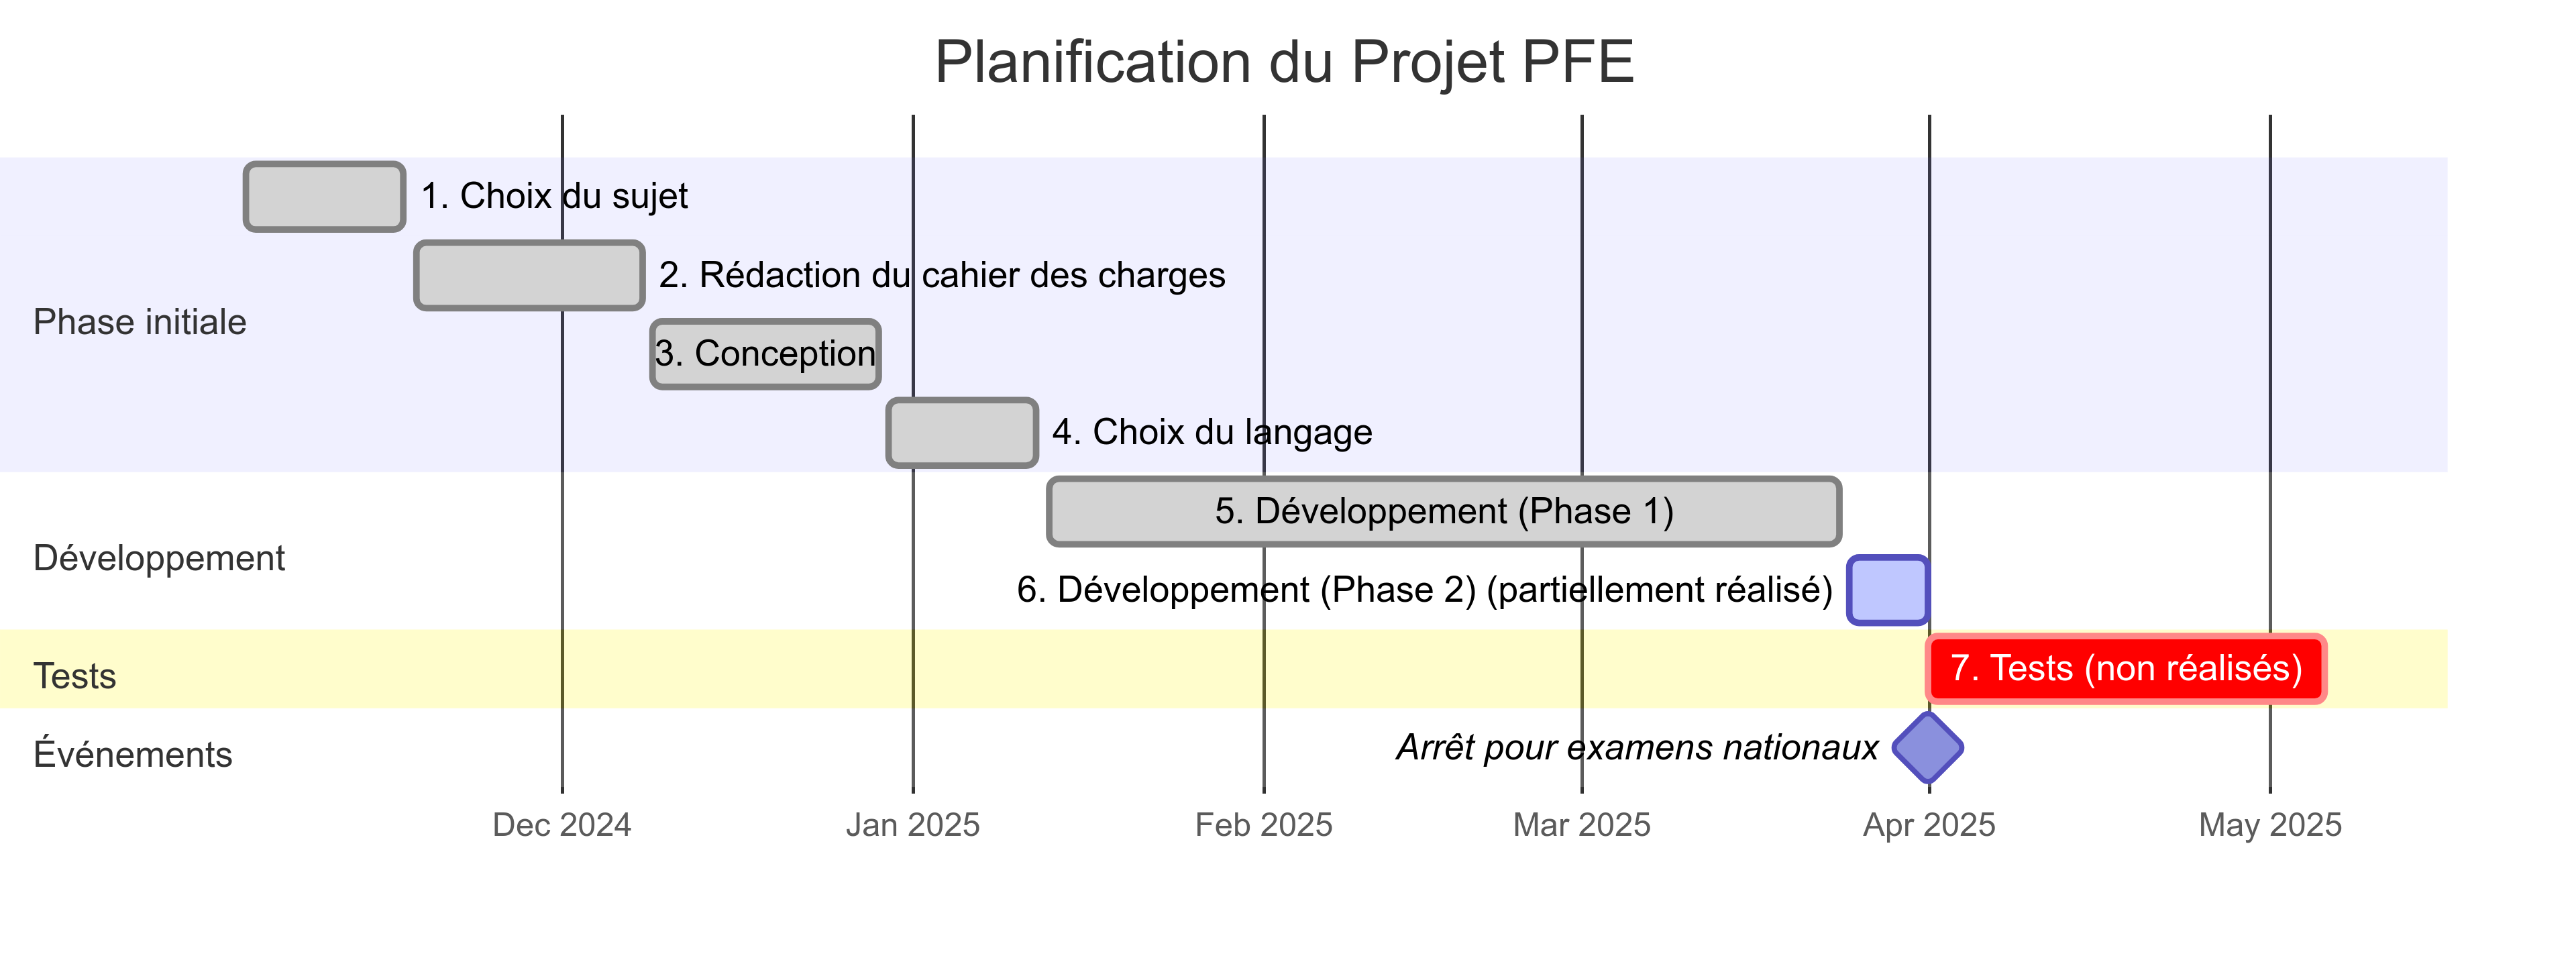
\includegraphics[width=1.0\textwidth,keepaspectratio]{pfe-pics/diagrames/Mermaid Chart - Create complex, visual diagrams with text. A smarter way of creating diagrams.-2025-06-10-203842.png}
  \caption{\textbf{Diagramme de Gantt} montrant la planification temporelle du projet.}
  \label{fig:gantt_chart}
\end{figure}

\subsection{Dépendances et chemin critique}

Le diagramme PERT ci-dessous illustre les dépendances entre les différentes tâches du projet et met en évidence le chemin critique:

\begin{figure}[H]
  \centering
  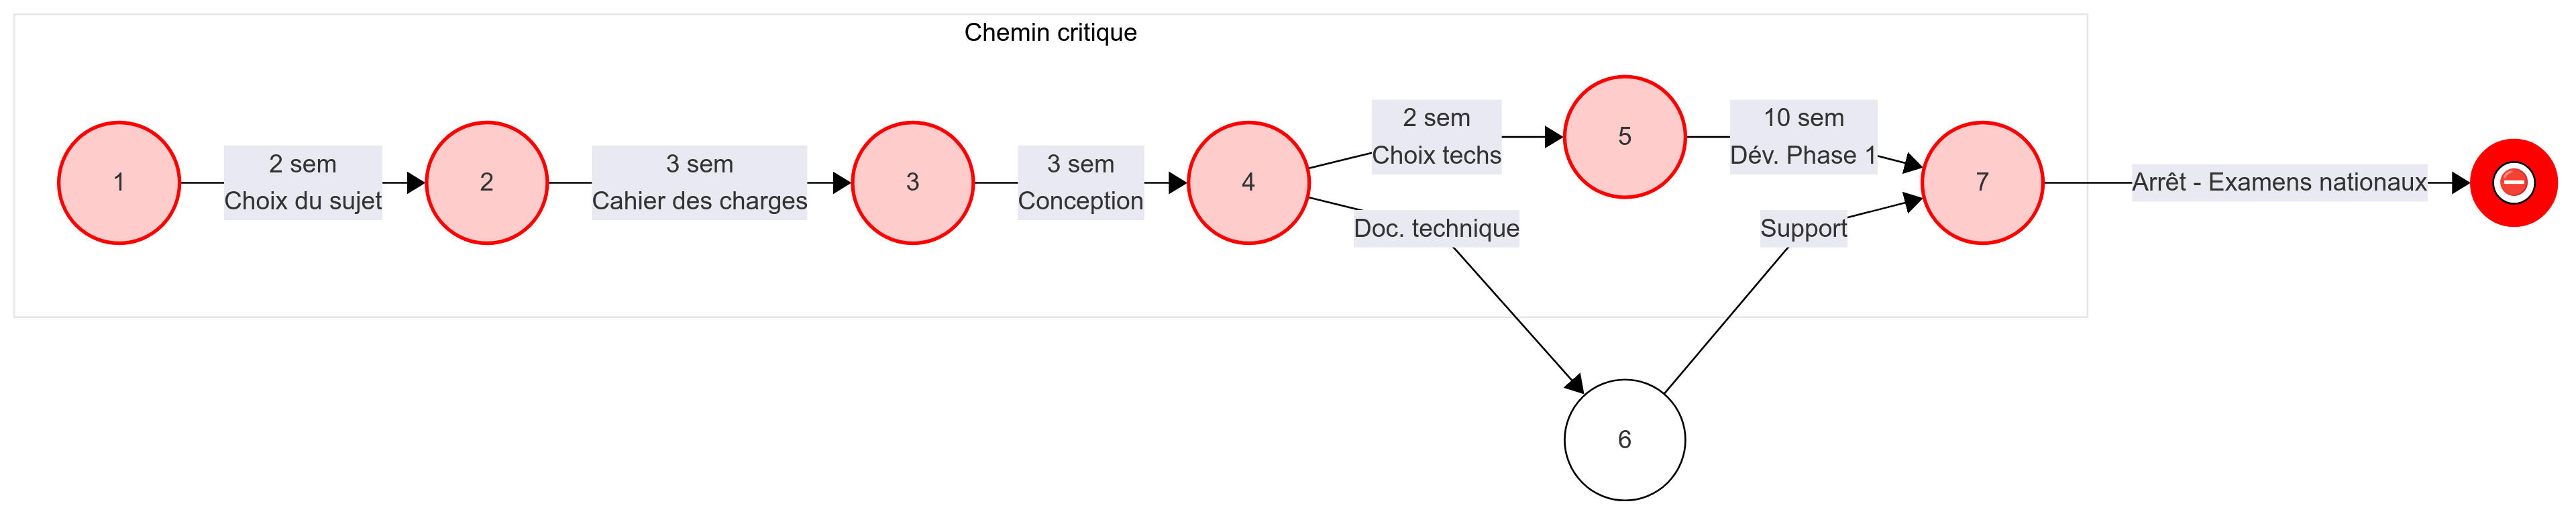
\includegraphics[width=1.0\textwidth,keepaspectratio]{pfe-pics/diagrames/Mermaid Chart - Create complex, visual diagrams with text. A smarter way of creating diagrams.-2025-06-10-203658.png}
  \caption{\textbf{Diagramme PERT} illustrant les dépendances et le chemin critique du projet.}
  \label{fig:pert_diagram}
\end{figure}

Ce diagramme met en évidence:

\begin{itemize}
  \item Les relations de précédence entre les activités
  
  \item Le chemin critique déterminant la durée minimale du projet
  
  \item Les marges disponibles pour certaines activités non critiques
  
  \item Les points de synchronisation nécessaires entre les différents volets du projet
\end{itemize}

\subsection{Répartition des tâches}

L'équipe de projet a été organisée selon les compétences de chaque membre:

\begin{itemize}
  \item \textbf{Architecture et conception}: Définition de l'architecture globale et des modèles de données
  
  \item \textbf{Développement backend}: Implémentation des API et services métier
  
  \item \textbf{Développement frontend web}: Création des interfaces utilisateur web
  
  \item \textbf{Développement mobile}: Réalisation des applications mobiles
  
  \item \textbf{Intelligence artificielle}: Conception et implémentation du système de profils IA
  
  \item \textbf{Tests et qualité}: Validation des fonctionnalités et correction des anomalies
  
  \item \textbf{Documentation}: Rédaction des guides et de la documentation technique
\end{itemize}

\section{Conclusion du cahier des charges}

Ce cahier des charges définit les contours de notre projet de fin d'études, qui vise à développer deux systèmes complémentaires pour moderniser l'environnement éducatif:

\begin{itemize}
  \item Un système de gestion scolaire complet couvrant les besoins administratifs et pédagogiques des établissements
  
  \item Une plateforme innovante de création de profils IA pour enrichir l'expérience d'apprentissage
\end{itemize}

L'approche choisie, combinant des technologies modernes et une méthodologie agile, permettra de livrer des solutions robustes, évolutives et adaptées aux besoins des différents utilisateurs. L'intégration des deux systèmes offrira une valeur ajoutée unique, positionnant ce projet à l'intersection de la gestion éducative traditionnelle et de l'innovation par l'intelligence artificielle.

Les spécifications détaillées dans ce document serviront de référence tout au long du développement, tout en permettant les ajustements nécessaires pour s'adapter aux retours des utilisateurs et aux contraintes techniques qui pourraient émerger. 